% =============================
%        CONFIGURACION
% =============================
\documentclass[spanish,12pt,letterpaper,oneside,titlepage]{report}

% Paquetes de fuentes
\usepackage[T1]{fontenc}
\usepackage[utf8]{inputenc}
\usepackage{lmodern}
\usepackage{tikz}
\usepackage{mathptmx}

% Configuración de la hoja
\usepackage[left=3cm, right=3cm, top=2.5cm, bottom=2.5cm]{geometry}
\usepackage{caption}

% Configuracion de imagenes
\usepackage{graphicx}
\usepackage{float}
\graphicspath{ {images/} }


% Configuracion de tablas
\usepackage[es-tabla]{babel}
\usepackage{tabularx}


% Configuracion de enlaces
\usepackage{xcolor}
\usepackage{hyperref}
\hypersetup{
	colorlinks=true,
	allcolors=blue
}

% Configuracion de referencias y citas
\usepackage{csquotes}
\usepackage[backend=biber,style=apa]{biblatex}
\addbibresource{referencias.bib}

% Configuracion de texto
\usepackage{titlesec}
\usepackage{setspace}
\onehalfspacing
\titlespacing*{\chapter}{0pt}{0pt}{20pt}
\setlength{\parindent}{0pt}
\titleformat{\chapter}
{\bfseries\fontsize{14}{16}\selectfont}
{\thechapter.}{1em}{}
\titleformat{\section}
{\bfseries\fontsize{14}{16}\selectfont}
{\thesection}{1em}{}

\usepackage{amssymb} % Paquete para fórmulas matemáticas

\usepackage{listings} % Paquete para escritura de código

% Configuracion notas de imagen y tabla
\captionsetup[figure]{
font={small},
labelfont=bf,
justification=centering
}
\captionsetup[table]{
font={small},
labelfont=bf,
justification=centering
}

% Configuracion del código 
\lstset{
    basicstyle=\ttfamily\small,     % Fuente
    backgroundcolor=\color{white},
    showstringspaces=false,         % Espacios
    frame=single,                   % Cuadro alrededor
    breaklines=true,                % Salto de línea automático
    captionpos=b                    % Caption abajo
}

\makeindex
\title{DESARROLLO DE APLICACIONES REACT PARA PLATAFORMA DEL SISTEMA INTEGRAL DE PRODUCCIÓN }
\author{Alejandro Martinez Rivera}


%--------------------------------------------------------------------
\begin{document}
% =============================
%           PORTADA
% =============================
\pagenumbering{roman}
\section*{Agradecimientos}

Quiero agradecer a mis \textbf{\textit{padres}}, ya que sin su apoyo incondicional durante todos estos años no hubiese podido llegar a ser quien soy ahora, dándome todo lo necesario y más para poder lograrlo.

A mi \textbf{\textit{padre}} le agradezco toda la fortaleza y perseverancia que me ha inculcado para seguir con mis metas y aspiraciones, sin importar las dificultades que estas puedan conllevar.

A mi \textbf{\textit{madre}} le agradezco la empatía y el amor por los demás que he aprendido de ella, permitiéndome así conocer a todas las personas que han llegado a mi vida y mantener lazos con ellas.

A mi \textbf{\textit{pareja}} le agradezco todo el apoyo y amor que me ha brindado en los momentos más difíciles y angustiosos, así como el tiempo que ha dedicado para estar a mi lado sin falta alguna.

A mis \textbf{\textit{amigos}}, que me han acompañado todos estos años, así como a los nuevos que he conocido en mi camino de vida, les agradezco por compartir experiencias y aprendizajes desde sus distintas perspectivas.

A mis \textbf{\textit{maestros}} les agradezco todo su tiempo y conocimientos, los cuales han contribuido a formarme como un futuro ingeniero, así como las experiencias de vida que han compartido más allá del ámbito educativo.

Al equipo de \textbf{\textit{Operational Planning IT}}, que en tan pocos meses me ha abierto las puertas para integrarme con ellos y brindarme sus conocimientos para formarme como profesionista desde mi periodo de residencias, confiando en mis capacidades. \newpage
\section*{Resumen}

El presente proyecto tuvo como objetivo el desarrollo e implementación de una aplicación web orientada al fortalecimiento del Sistema Integral de Producción (SIP) de TenarisTamsa, con la finalidad de optimizar la gestión de la información dentro de las áreas de producción y ensamblaje. La propuesta surgió a partir de la necesidad de reducir las limitaciones existentes derivadas del uso de registros manuales, la fragmentación de la información y la falta de integración entre distintos sistemas utilizados en el entorno industrial.


Para atender esta problemática, se diseñó una solución tecnológica basada en una arquitectura moderna de software, utilizando React.js para el desarrollo del frontend, .NET y C\# para la lógica de negocio en el backend, así como PostgreSQL como sistema gestor de bases de datos. La solución fue desarrollada bajo una arquitectura de N-Capas para el backend y una arquitectura basada en componentes para el frontend, permitiendo la modularidad, reutilización y mantenibilidad del sistema.


Durante el desarrollo del proyecto se implementaron distintos módulos funcionales orientados a cubrir las necesidades operativas del SIP, entre los que destacan el inicio de sesión, la gestión de usuarios, el reporte y gestión de producción, el control de almacén, la visualización de información productiva y la programación de órdenes de producción. Asimismo, se integraron mecanismos de autenticación, control de acceso basado en roles, manejo multiusuario e integridad de la información, garantizando la seguridad y confiabilidad del sistema.


Como resultado, se obtuvo una aplicación web capaz de centralizar información, digitalizar procesos operativos y facilitar el acceso a datos en tiempo real, contribuyendo a mejorar la trazabilidad, el control y la toma de decisiones dentro de la organización. Además, el proyecto permitió aplicar conocimientos relacionados con el desarrollo de software, arquitecturas web y buenas prácticas de ingeniería, fortaleciendo tanto la experiencia profesional como las capacidades tecnológicas orientadas a entornos industriales de alta demanda.
 \newpage
\tableofcontents
\newpage
\listoffigures
\newpage
\listoftables
\newpage
\pagenumbering{arabic}

\chapter{Introducción}

La transformación digital en los entornos industriales ha impulsado la necesidad de desarrollar soluciones tecnológicas que optimicen la gestión de la información, mejoren la eficiencia operativa y faciliten la toma de decisiones estratégicas. En este contexto, las organizaciones que dependen de procesos productivos complejos requieren sistemas informáticos capaces de integrarse de manera efectiva, garantizar la disponibilidad de datos en tiempo real y asegurar la trazabilidad de sus operaciones.

El presente documento tiene como propósito describir el desarrollo de una solución tecnológica orientada a fortalecer el Sistema Integral de Producción dentro del entorno industrial de TenarisTamsa. A partir del análisis de la problemática existente, se identifican diversas limitaciones relacionadas con la gestión manual de información, la falta de integración entre sistemas y la necesidad de contar con herramientas que permitan un mejor control y seguimiento de los procesos productivos.

Con base en lo anterior, se plantea el diseño e implementación de una aplicación web que permita digitalizar procesos, centralizar la información y mejorar la interacción de los usuarios con el sistema, utilizando tecnologías modernas de desarrollo tanto en el front-end como en el back-end. Esta propuesta busca no solo atender las necesidades actuales de la organización, sino también sentar las bases para la escalabilidad y mejora continua de sus sistemas informáticos.

Este trabajo refleja la aplicación de conocimientos teóricos y prácticos en un entorno real, contribuyendo al desarrollo de soluciones tecnológicas que impactan directamente en la eficiencia y competitividad de la organización.

\chapter{Marco metodológico}
\section{Caracterización de la empresa}

\subsection{Información general}

TenarisTamsa es el Centro Industrial de Tenaris en México, con más de 70 años de operación, consolidándose como uno de los complejos industriales más grandes del mundo dedicados a la fabricación de tubos de acero sin costura y accesorios. Sus productos atienden a sectores como la industria energética, automotriz, minera, industrial y de construcción.

Además, la empresa ha participado en proyectos altamente exigentes de exploración y producción de petróleo, incluyendo aguas profundas y yacimientos no convencionales.

Asimismo, TenarisTamsa cuenta con un Centro de Investigación y Desarrollo único en México, realizando investigaciones avanzadas en metalurgia, procesos y ensayos de escala real.
Fuente: \parencite{TenarisAboutUs}

\begin{figure}[h]
    \centering
    
\includegraphics[width=0.6\linewidth]{tenarisLogo.png}
    \caption{Logotipo de TenarisTamsa}
    \label{fig:TamsaLogo}
\end{figure}

\subsection{Identidad corporativa}

A nivel global, Tenaris es el fabricante líder de tubos y servicios relacionados para la industria energética y diversas aplicaciones industriales. Su sistema de producción integra procesos de fabricación de acero, laminado, conformado, tratamiento térmico, roscado y acabado, con instalaciones en 17 países y una red de I+D en constante innovación.

Como organización, busca mantener los más altos estándares de seguridad, calidad, desempeño e innovación, trabajando estrechamente con sus clientes a través de soluciones integradas como Rig Direct®, las cuales optimizan toda la cadena de suministro.

La identidad corporativa de Tenaris se fundamenta en:
\begin{itemize}
    \item Excelencia operativa e industrial.
    \item Innovación continua en productos y servicios.
    \item Presencia global con capacidad de respuesta local.
    \item Fuerte enfoque en seguridad, calidad y desempeño.
\end{itemize}

\subsection{Valores organizacionales}

Tenaris define un conjunto de valores que orientan su cultura y desempeño (tabla \ref{tab:valores}):

\begin{table}[H]
    \centering
    \caption{Valores de TenarisTamsa.}
    \label{tab:valores}
    \begin{tabularx}{\textwidth}{|X|X|}
        \hline
        Valores                           & Descripción                                                                                                                                                                                                                                                \\ \hline
        Salud, Seguridad y Ambiente (HSE) & La seguridad es la prioridad principal de la empresa. Tenaris considera que todas las lesiones laborales pueden y deben ser evitadas. Además, invierte constantemente en tecnologías para reducir el impacto ambiental y mejorar sus procesos sostenibles. \\ \hline
        Protección ambiental              & Las plantas de Tenaris operan bajo estrictos estándares de cuidado ambiental, incorporando innovaciones tecnológicas para minimizar emisiones, residuos e impactos operativos.                                                                             \\ \hline
        Transparencia                     & La empresa promueve una cultura de integridad, asegurando relaciones transparentes con accionistas, empleados, clientes, proveedores y comunidades.                                                                                                        \\ \hline
        Comunidad y sustentabilidad       & Tenaris impulsa programas comunitarios, educativos y ambientales, además de publicar reportes transparentes de seguridad, salud y ambiente como parte de su responsabilidad corporativa.                                                                   \\ \hline
    \end{tabularx}
\end{table}

Fuente: \parencite{Tenaris} \newpage
\section{Problemática}

En las áreas de producción y ensamblaje de TenarisTamsa se utiliza diariamente el Sistema Integral de Producción para el seguimiento y la planificación de los pedidos de las distintas gamas de productos que la empresa provee a sus clientes. Este sistema permite gestionar información relacionada con los procesos productivos, facilitando la organización de pedidos y el monitoreo de las diferentes etapas de fabricación.

No obstante, debido al crecimiento constante de la empresa y a su expansión como proveedor para diversos clientes, los requerimientos operativos dentro del área productiva se han vuelto cada vez más complejos. Entre estos requerimientos se encuentran la necesidad de contar con información actualizada en tiempo real, la trazabilidad completa de los pedidos, la integración de datos entre distintas áreas y plantas, así como la capacidad de analizar información histórica para la toma de decisiones y la mejora continua de los procesos.

Sin embargo, el sistema actualmente utilizado presenta diversas limitaciones que dificultan el cumplimiento de dichos requerimientos operativos. Una de las principales limitaciones es el uso de registros manuales en papel por parte de los trabajadores, lo que incrementa el riesgo de errores, pérdida de información y retrasos en la actualización de los datos. Asimismo, existen múltiples sistemas de información que operan de manera independiente, sin una integración adecuada, lo que obliga a consultar diferentes fuentes por separado y dificulta la consolidación y análisis de la información.

Adicionalmente, al formar parte del grupo corporativo Techint Group, la empresa requiere mantener homogeneidad en los sistemas utilizados por las diferentes plantas del grupo, tales como TenarisSiderca y TenarisDalmine, entre otras, las cuales realizan procesos similares. Este contexto implica como requerimiento operativo la interoperabilidad entre sistemas y la estandarización de la información.

No obstante, los sistemas actuales no permiten una integración eficiente con las plantas previamente mencionadas, lo que limita el intercambio oportuno de información, especialmente en situaciones relacionadas con la mejora de procesos o la prevención de problemas potenciales en otras instalaciones.

En consecuencia, surge la necesidad de analizar y desarrollar soluciones que permitan optimizar la gestión de la información dentro de los procesos productivos, reducir las limitaciones actuales y cumplir con los requerimientos operativos de integración, trazabilidad y disponibilidad de la información, así como garantizar la interoperabilidad de los sistemas entre las distintas plantas del grupo. \newpage
\section{Propuesta de solución}

Con base en la problemática anteriormente planteada, se propone el desarrollo de un sistema de aplicación web (WebApp) que se integre al ecosistema del Sistema Integral de Producción, con el objetivo de optimizar la gestión de la información y mejorar la eficiencia de los procesos operativos dentro de las áreas de producción y ensamblaje.

La solución propuesta busca atender directamente las limitaciones identificadas, principalmente la dependencia de registros manuales en papel y la existencia de sistemas de información no integrados. Para ello, el sistema permitirá la digitalización de los procesos de captura de datos en planta, reduciendo errores humanos, evitando la pérdida de información y garantizando la disponibilidad de los datos en tiempo real.

Asimismo, el sistema estará diseñado para centralizar la información proveniente de distintas fuentes, permitiendo su integración en una única plataforma. Esto facilitará la consulta, el análisis y la trazabilidad completa de los pedidos a lo largo de todas las etapas del proceso productivo, atendiendo así los requerimientos operativos de visibilidad y control.

Dentro del marco tecnológico, se propone el uso de React.js como librería para el desarrollo de interfaces de usuario dinámicas e intuitivas, facilitando la interacción del personal operativo con el sistema y permitiendo su escalabilidad ante futuros requerimientos. Por otra parte, se plantea el uso de tecnologías del ecosistema .NET, empleando C\# para la lógica de negocio, lo cual permitirá implementar una arquitectura robusta, mantenible y alineada con los recursos tecnológicos disponibles en la organización.

Para la gestión de datos, se propone el uso de PostgreSQL como sistema de bases de datos, debido a su capacidad para manejar grandes volúmenes de información, garantizar la integridad de los datos y ofrecer un alto rendimiento en consultas, lo que resulta fundamental para cumplir con los requerimientos de acceso oportuno y análisis de información.

En conjunto, esta solución permitirá mejorar la administración de la información, agilizar los procesos de seguimiento y control, garantizar la trazabilidad de los pedidos, reducir la dependencia de procesos manuales y fortalecer la toma de decisiones mediante el acceso a información confiable y oportuna. \newpage
\section{Objetivos}

\subsection{Objetivo general}

Desarrollar una aplicación web utilizando tecnologías emergentes que fortalezca las funcionalidades del Sistema Integral de Producción (SIP), permitiendo visualizar, proyectar y analizar información crítica relacionada con las órdenes de producción, con el fin de mejorar la precisión en la planificación, facilitar la detección temprana de riesgos y optimizar la capacidad operativa del sistema.

\subsection{Objetivos específicos}

\begin{enumerate}
    \item Analizar la arquitectura, el flujo de información y los lineamientos tecnológicos del Sistema Integral de Producción (SIP) con el propósito de asegurar una adecuada integración de los nuevos desarrollos con la plataforma existente.

    \item Diseñar e implementar componentes y vistas utilizando React.js que permitan consultar, filtrar y visualizar información relevante del proceso productivo, incluyendo proyecciones, estados y posibles riesgos asociados a las órdenes de producción.

    \item Integrar los componentes desarrollados con las fuentes de datos del sistema mediante el consumo de servicios, gestionando adecuadamente estados de carga, manejo de errores y actualización de la información.

    \item Mejorar la experiencia de usuario mediante el desarrollo de interfaces claras, estructuradas y alineadas con las necesidades operativas de planificación y control dentro del entorno productivo.

    \item Aplicar buenas prácticas de desarrollo de software, documentación y estandarización del código, con el fin de garantizar la mantenibilidad, escalabilidad y evolución futura de los módulos desarrollados dentro del SIP.
\end{enumerate} \newpage
\section{Justificación}

La implementación de una aplicación web integrada al Sistema Integral de Producción representa una respuesta directa y fundamentada a las limitaciones operativas identificadas en el área de producción y ensamblaje de TenarisTamsa.

En primer lugar, la digitalización de los procesos de captura de datos en planta elimina la dependencia de registros manuales en papel, reduciendo significativamente el riesgo de errores humanos, la pérdida de información y los retrasos en la actualización de datos. Al garantizar la disponibilidad de la información en tiempo real, el personal operativo podrá consultar el estado actual de los procesos productivos de manera inmediata y confiable, mejorando la capacidad de respuesta ante contingencias y facilitando la toma de decisiones oportuna.

En segundo lugar, la centralización de la información proveniente de distintas fuentes en una única plataforma resuelve la fragmentación actual de los sistemas, eliminando la necesidad de consultar múltiples fuentes de manera independiente. Esto permite consolidar y analizar la información de forma integrada, brindando trazabilidad completa sobre las órdenes de producción a lo largo de todas las etapas del proceso, lo cual resulta fundamental para la mejora continua y el control operativo.

Asimismo, al desarrollar el sistema bajo un stack tecnológico moderno y estandarizado, se sientan las bases para garantizar la interoperabilidad entre las distintas plantas del grupo Techint, como TenarisSiderca y TenarisDalmine. Esta homogeneidad tecnológica facilita el intercambio oportuno de información entre instalaciones, tanto para la mejora de procesos como para la prevención de problemas productivos en el conjunto de la organización.

Finalmente, la solución contribuye a fortalecer la escalabilidad y mantenibilidad de los sistemas informáticos de TenarisTamsa, alineándose con su modelo de excelencia operativa e innovación continua. Al reducir la dependencia de procesos manuales y proporcionar herramientas de visualización, proyección y análisis de información crítica, la organización estará mejor posicionada para atender el crecimiento constante de sus requerimientos operativos y para sostener su competitividad como proveedor de clase mundial. \newpage
\section{Descripción del área de desarrollo}

El área de Operational Planning IT tiene como objetivo coordinar y optimizar los procesos de planeación relacionados con los sistemas informáticos que soportan las operaciones industriales de TenarisTamsa. Su función principal es asegurar que las soluciones tecnológicas estén alineadas con los objetivos operativos de la planta y contribuyan a mejorar la eficiencia, confiabilidad y calidad de los procesos productivos. 

El área de Operational Planning IT es estratégica en un entorno industrial altamente automatizado como TenarisTamsa. Su labor garantiza que:

\begin{itemize}
    \item Los sistemas operativos y de producción trabajen con continuidad, estabilidad y eficiencia.
    \item Las mejoras tecnológicas tengan un impacto medible en la calidad, seguridad y productividad.
    \item La empresa mantenga un enfoque preventivo y predictivo en la gestión de TI.
\end{itemize}

 Dado el nivel de automatización y la integración tecnológica presente en TenarisTamsa, este equipo contribuye directamente al ambiente de excelencia operativa que caracteriza a la compañía. \newpage
\section{Planificación de actividades}

Las actividades planificadas y realizadas durante el periodo de residencias enero-junio del 2026 son las que se describen a continuación. En la figura \ref{fig:Cronograma} se observa el tiempo designado para cada fase y un avance real hasta la entrega de este reporte.

Fase 1: Familiarización con el entorno, el SIP y el stack tecnológico
\begin{itemize}
    \item Inducción al área y revisión de procesos internos.
    \item Exploración de la arquitectura general del SIP y sus módulos principales.
\end{itemize}

Fase 2: Prácticas iniciales de React y construcción de componentes básicos
\begin{itemize}
    \item Repaso de conceptos esenciales: hooks, estados, props.
    \item Construcción de componentes simples.
\end{itemize}

Fase 3: Implementación de componentes reutilizables orientados al SIP
\begin{itemize}
    \item Identificación de componentes candidatos: tablas, formularios, modales, filtros.
    \item Integración de estilos estandarizados (temas, tipografías, espaciados).
\end{itemize}

Fase 4: Desarrollo de vistas funcionales dentro del SIP
\begin{itemize}
    \item Maquetado inicial de pantallas usando componentes creados.
    \item Implementación de lógica de negocio local (validaciones, comportamientos).
    \item Integración de componentes reutilizables dentro del flujo real de las vistas.
\end{itemize}

Fase 5: Integración con servicios y manejo de datos reales o simulados
\begin{itemize}
    \item Consumo de APIs: fetch, manejo de errores.
    \item Pruebas de conexión en entornos de desarrollo.
    \item Verificación con datos reales y retroalimentación con el área funcional.
\end{itemize}

Fase 6: Ajustes, pruebas, mejoras visuales y refinamiento general
\begin{itemize}
    \item Corrección de errores detectados durante QA interno.
    \item Mejoras visuales.
\end{itemize}

Fase 7: Documentación y presentación de avances del proyecto
\begin{itemize}
    \item Elaboración de documentación técnica final (componentes, vistas, APIs usadas).x
    \item Demostración del proyecto final.
\end{itemize}

Estas actividades aseguran la entrega de una solución tecnológica robusta, moderna y alineada con las necesidades operativas de la organización.
\begin{figure}[h]
    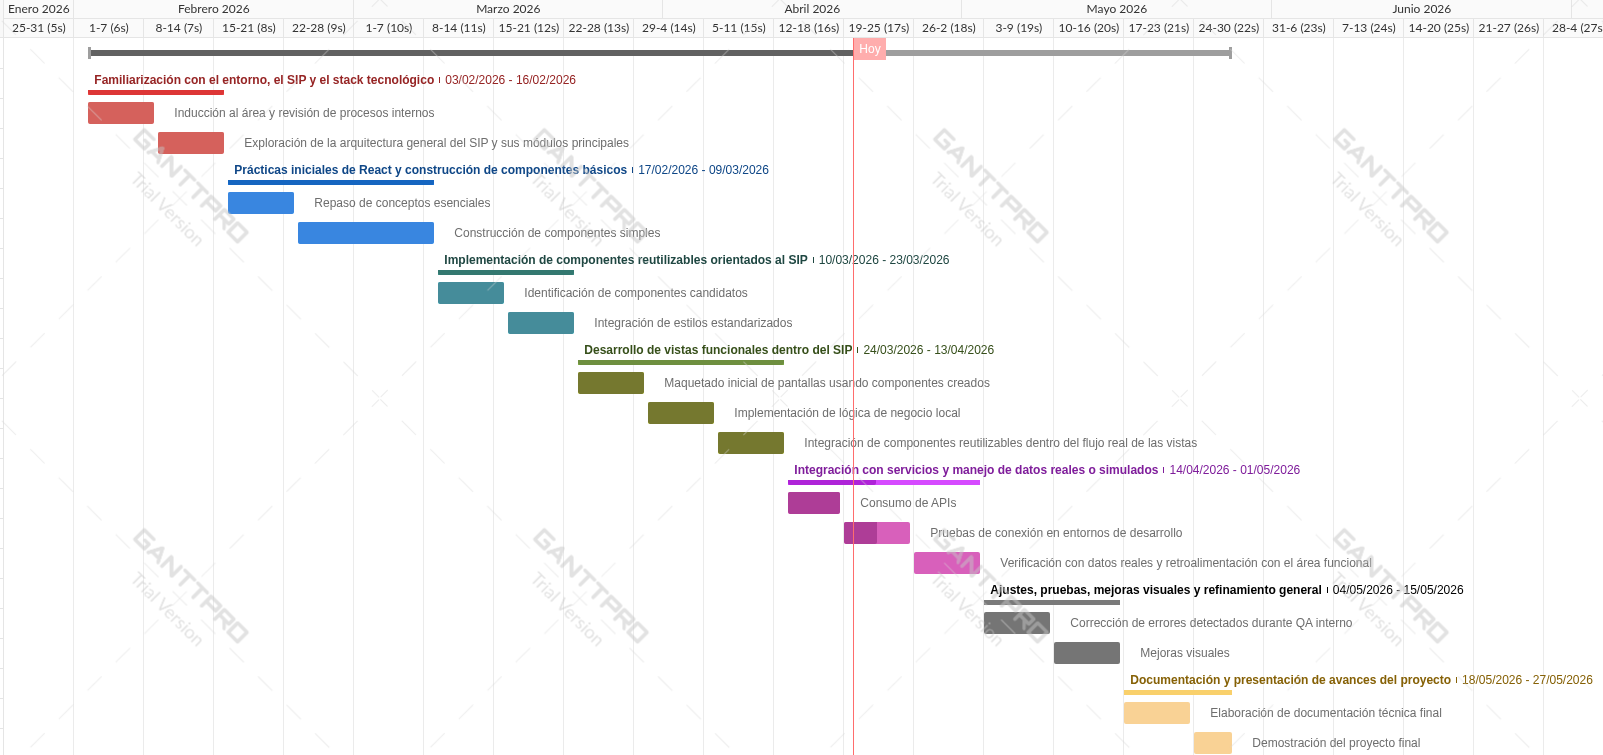
\includegraphics[width=1\linewidth]{cronograma.png}
    \caption{Cronograma de trabajo.}
    \label{fig:Cronograma}
\end{figure}
 \newpage

\chapter{Marco teórico}
\section{Front-end}

El desarrollo front-end se refiere al proceso de diseño, estructuración e implementación de las interfaces visuales con las que los usuarios interactúan dentro de un sistema. Su propósito principal es facilitar la interacción entre el usuario y las funcionalidades del sistema, permitiendo ejecutar acciones previamente definidas de manera intuitiva y eficiente \parencite{FrontentGG}.

Este proceso implica considerar diversos factores, tales como los dispositivos en los que se visualizará el sistema, así como los entornos de ejecución, en el caso de las aplicaciones web (WebApps). Asimismo, el desarrollo front-end promueve la creación de componentes reutilizables, lo que contribuye a evitar la duplicidad de código y optimiza tanto el mantenimiento como la escalabilidad del sistema.


% =======================
% |   LENGUAJES WEB     |
% =======================
\subsection{Lenguajes de desarrollo web}

Los lenguajes de desarrollo web son aquellos diseñados específicamente para la creación de sistemas que operan en entornos web, los cuales pueden ser procesados e interpretados por los navegadores o servidores. Estos lenguajes permiten construir aplicaciones accesibles a través de internet, integrando tanto la presentación como la lógica del sistema.

Dentro del desarrollo web se distinguen dos componentes principales: el front-end, que corresponde a la parte del sistema que se ejecuta en el navegador y con la que el usuario interactúa directamente, y el back-end, que se ejecuta en el servidor y se encarga de la lógica de negocio, el procesamiento de datos y la comunicación con bases de datos. Entre los lenguajes fundamentales del desarrollo web se encuentran HTML, CSS y JavaScript \ref{fig:LenguajesWeb}.

\begin{figure}[h]
  \centering
  
\includegraphics[width=0.6\linewidth]{lenguajesWeb.png}
  \caption{Lenguajes de desarrollo web.}
  \label{fig:LenguajesWeb}
\end{figure}


% =======================
% |        HTML         |
% =======================
\subsubsection{HTML (HyperText Markup Language)}

Es el lenguaje de marcado estándar utilizado para la estructuración y maquetación de páginas web. Permite definir la organización del contenido que será interpretado por los navegadores, constituyendo la base sobre la cual se construyen las interfaces de usuario en aplicaciones web \parencite{HTMLmdn}.

Se hace uso de etiquetas (tags) (Ver ejemplo \ref{lst:ejeHTML}), las cuales delimitan los distintos elementos de la página. En su mayoría, estas etiquetas están compuestas por una etiqueta de apertura y una de cierre, aunque existen algunas etiquetas autocontenidas. Cada elemento puede incluir atributos que proporcionan información adicional o configuran su comportamiento.

Estos atributos permiten la integración y manipulación de los elementos HTML a través de otros lenguajes complementarios como CSS (Cascading Style Sheets), encargado de la presentación visual, y JavaScript, responsable de la interactividad y la lógica del lado del cliente.

\begin{lstlisting}[language=HTML, caption={Ejemplo de código HTML.}, label={lst:ejeHTML}]
<html lang="en">
<head>
    <meta charset="UTF-8">
    <meta name="viewport" content="width=device-width, initial-scale=1.0">
    <title>Pagina web</title>
</head>
<body>
   <div>
    <img src="img.jpg" alt="imagen de prueba" />
   </div> 
</body>
</html>
\end{lstlisting}

% =======================
% |         CSS         |
% =======================

\subsubsection{CSS (Cascading Style Sheets)}

Es el lenguaje utilizado para definir la presentación visual de los elementos estructurados mediante HTML en una página web. Permite aplicar estilos como colores, tipografías, tamaños, márgenes, alineaciones y posicionamiento, con el objetivo de mejorar la apariencia y la experiencia de usuario en la interfaz \parencite{CSSmdn}.

La aplicación de estilos en CSS se realiza mediante selectores, los cuales permiten identificar elementos HTML a través de nombres de etiqueta, clases, identificadores u otros atributos (ejemplo \ref{lst:ejeCSS}). A partir de estos selectores, se definen reglas de estilo compuestas por propiedades y valores que determinan la apariencia de cada elemento.

CSS puede implementarse de distintas formas: de manera interna, dentro del mismo archivo HTML; en línea, directamente sobre los elementos; o de forma externa, mediante archivos independientes con extensión .css que se enlazan al documento HTML. Esta última forma favorece la reutilización de estilos y la organización del código en proyectos de mayor escala.

\begin{lstlisting}[language=HTML, caption={Ejemplo de código CSS.}, label={lst:ejeCSS}]
body {
  background-color: lightblue;
}
.titulo {
  color: white;
  text-align: center;
}
#paragraph {
  font-family: verdana;
  font-size: 20px;
}
\end{lstlisting}

% =======================
% |     JAVASCRIPT      |
% =======================

\subsubsection{JavaScript}

Es un lenguaje de programación utilizado en el desarrollo web para dotar de funcionalidad e interactividad a los elementos de una página. Permite implementar comportamientos dinámicos mediante la definición de eventos que se activan en respuesta a las acciones del usuario, como clics, desplazamientos o la introducción de datos \parencite[]{JSmdn}.

A través de JavaScript, es posible manipular el contenido y la estructura del documento HTML en tiempo real, así como controlar la navegación entre secciones, validar formularios, gestionar sesiones de usuario e interactuar con servicios externos mediante el intercambio de datos con servidores.

Este lenguaje se ejecuta principalmente en el navegador del cliente, aunque también puede emplearse en el lado del servidor mediante entornos de ejecución específicos. Su integración con HTML y CSS lo convierte en un componente fundamental para el desarrollo de aplicaciones web modernas.

\subsection{React.js}

React.js es una biblioteca de código abierto desarrollada por Meta Platforms, Inc. (anteriormente Facebook), utilizada para la construcción de interfaces de usuario en aplicaciones web. Se basa en el uso de componentes, los cuales son unidades independientes y reutilizables que permiten estructurar la interfaz de manera modular, facilitando el desarrollo, mantenimiento y escalabilidad de los sistemas.

Esta biblioteca emplea JavaScript y, de forma opcional, TypeScript, integrando una extensión de sintaxis conocida como JSX (o TSX en el caso de TypeScript). Esta sintaxis permite combinar estructuras similares a HTML con la lógica de programación, lo que posibilita una definición más intuitiva de la interfaz y su comportamiento en un mismo contexto.

La filosofía principal de React.js se centra en la creación de componentes reutilizables y atómicos que gestionan su propio estado (state) y propiedades (props), permitiendo que la interfaz de usuario se actualice de manera eficiente en respuesta a cambios en los datos. Este enfoque declarativo favorece el desarrollo de aplicaciones dinámicas, donde los elementos visuales pueden modificar su comportamiento e interacción según las necesidades del sistema.

\begin{figure}[ht]
    \centering
    
\includegraphics[width=0.3\linewidth]{teorico/react.png}
    \caption{Logo de React.js.}
    \label{fig:LogoReact}
\end{figure}

\subsection{Vite}

Vite es una herramienta moderna de desarrollo y construcción de aplicaciones web que facilita la ejecución, compilación y optimización del código en proyectos basados en frameworks como React. Su principal objetivo es mejorar tanto la experiencia de desarrollo como el rendimiento de las aplicaciones finales que se ejecutan en el navegador.

Vite se caracteriza por ofrecer un entorno de desarrollo rápido mediante el uso de módulos nativos del navegador, lo que permite cargar únicamente las dependencias necesarias bajo demanda. Esto contribuye a reducir los tiempos de inicio y a optimizar el consumo de recursos, evitando la carga de código innecesario. Además, durante el proceso de construcción (build), Vite genera versiones optimizadas del código, preparadas para su despliegue en entornos de producción \parencite[]{ViteJS}.

Una de sus principales características es el soporte de Hot Module Replacement (HMR), que permite reflejar en tiempo real los cambios realizados en el código sin necesidad de recargar completamente la aplicación. Esto mejora significativamente la eficiencia del desarrollo (Figura \ref{fig:Vitejs}).

\begin{figure}[ht]
    \centering
    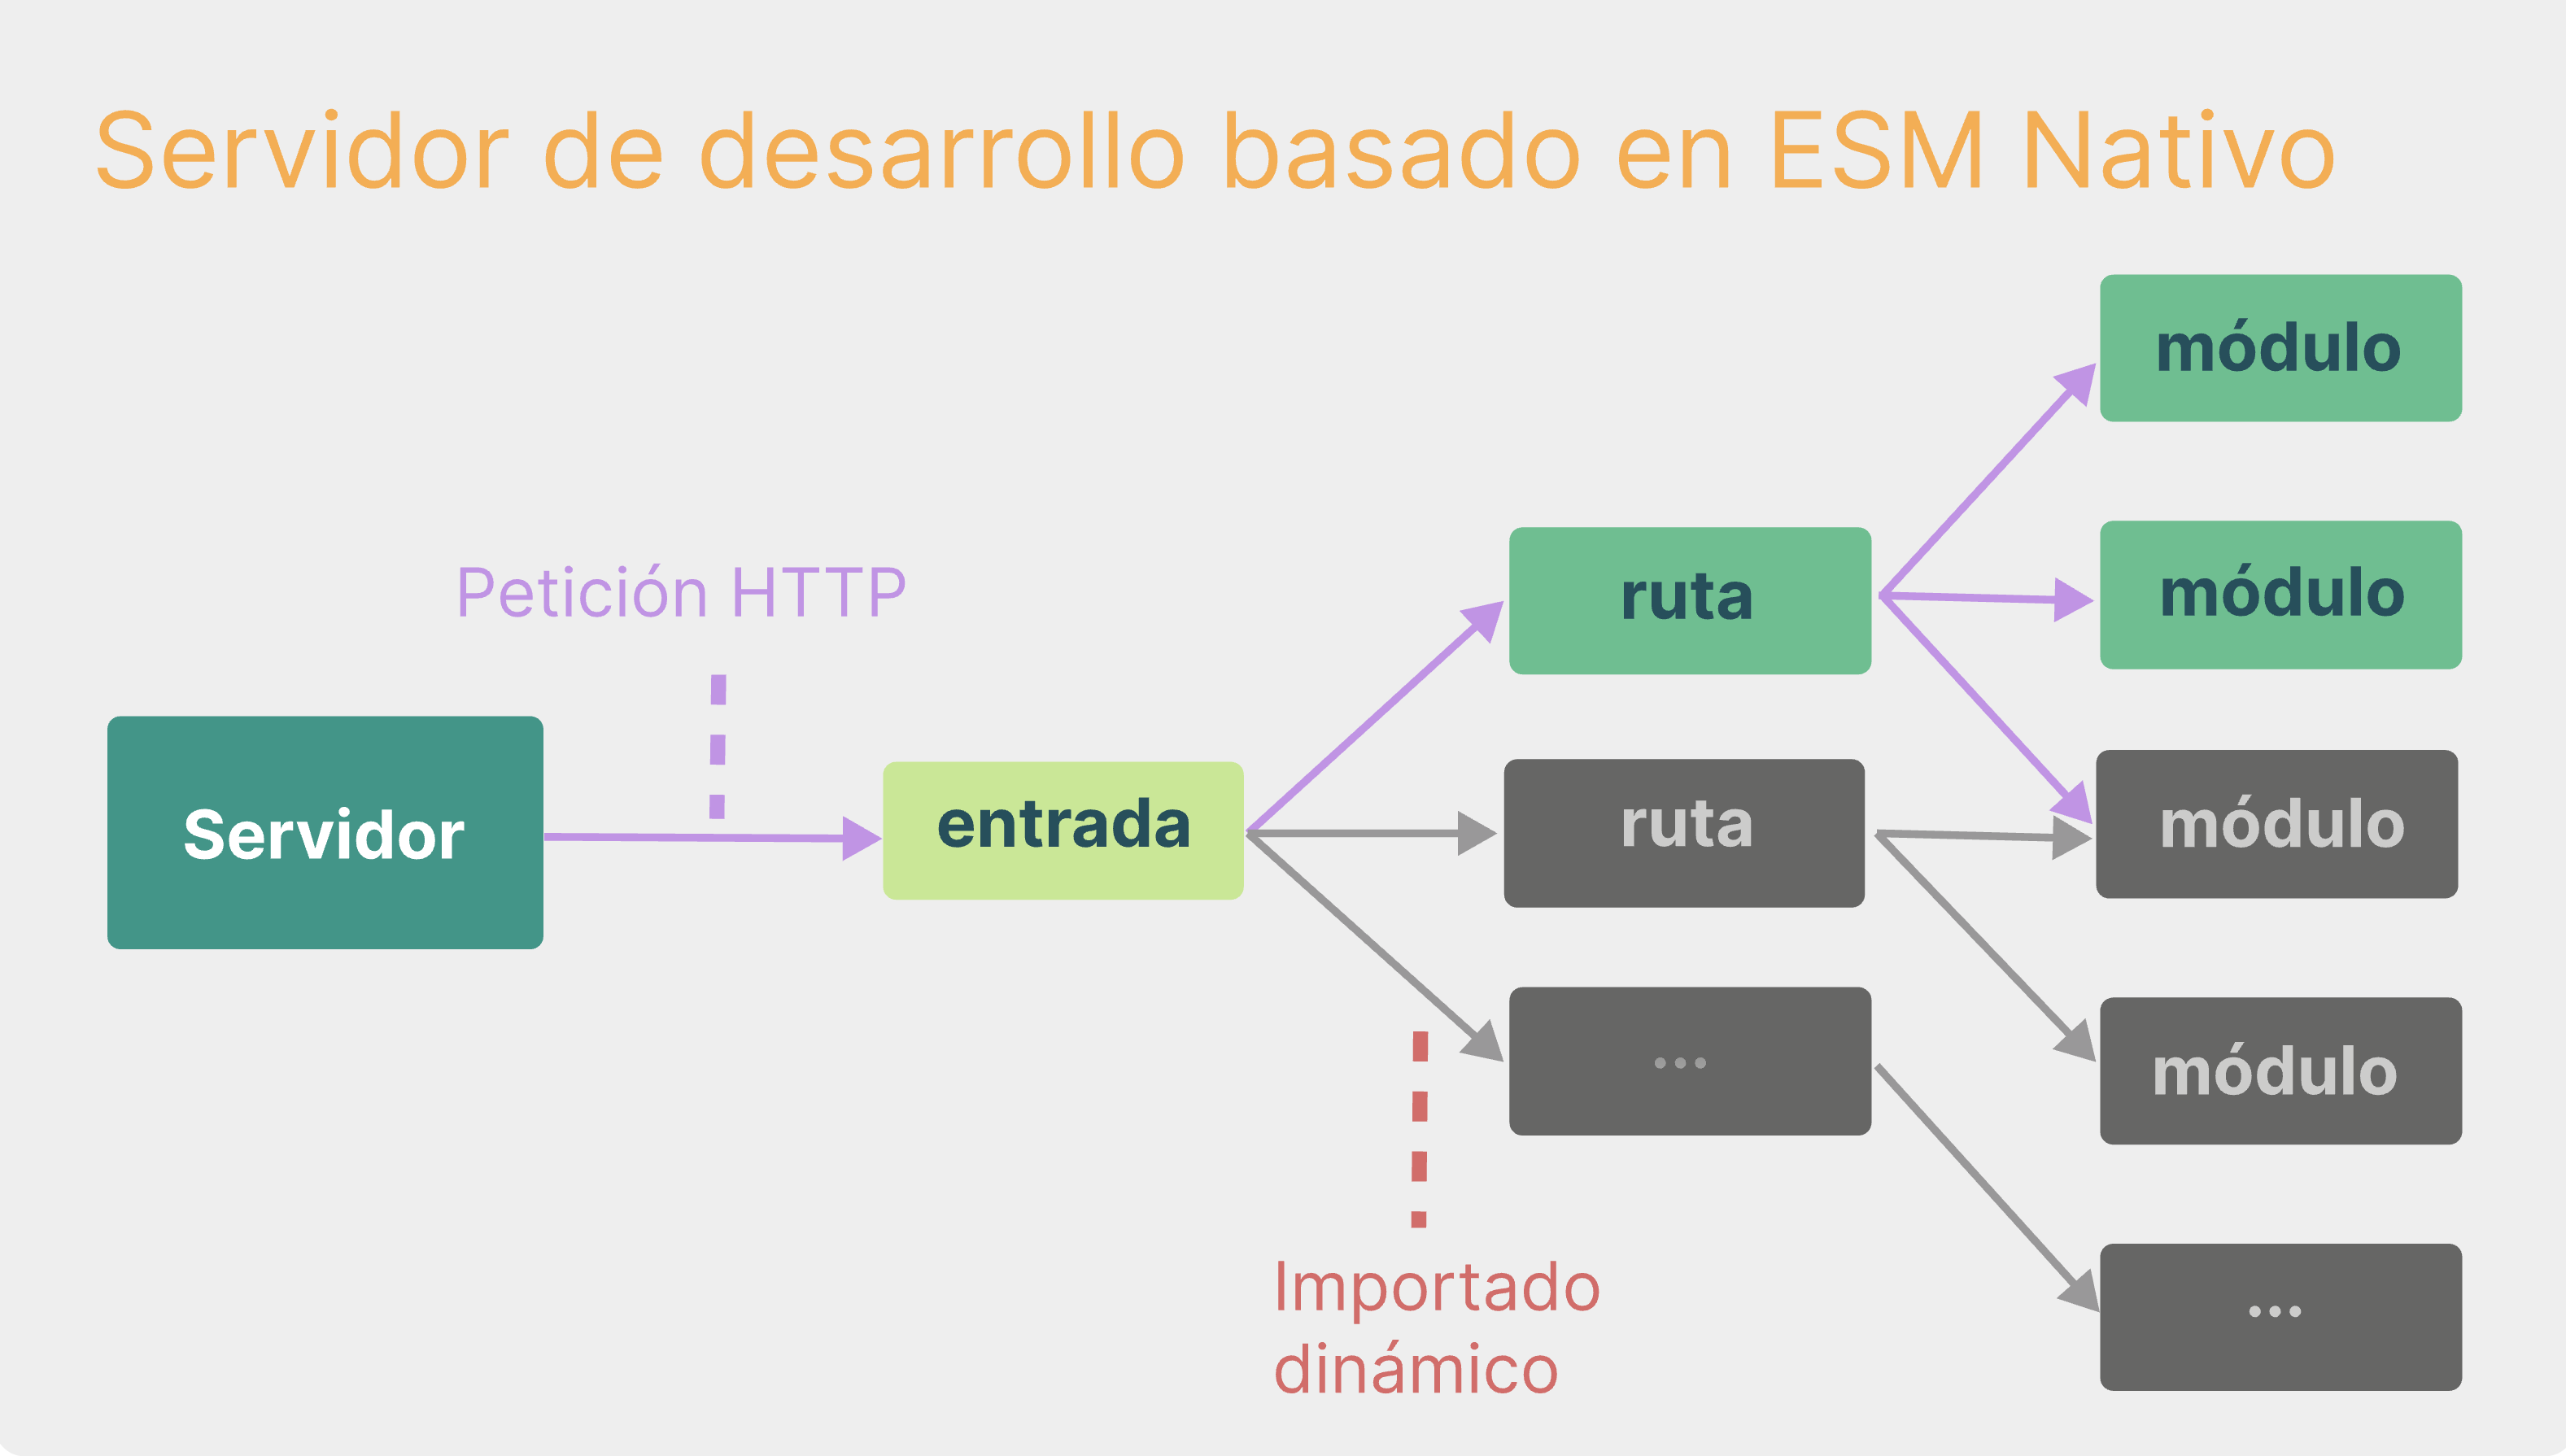
\includegraphics[width=0.7\linewidth]{teorico/vitejs.png}
    \caption{Funcionalidad de Vitejs.}
    \label{fig:Vitejs}
\end{figure}

A diferencia de herramientas tradicionales como Babel, que se enfocan principalmente en la transformación de código, Vite integra un enfoque más completo que abarca tanto el desarrollo como la optimización del sistema, posicionándose como una alternativa moderna ampliamente adoptada en la comunidad de desarrollo web \parencite[]{BuildTools}.

\subsection{Nodejs}

Node.js es un entorno de ejecución de JavaScript, de código abierto y multiplataforma, que permite ejecutar código fuera del navegador, principalmente en el lado del servidor. Se caracteriza por su modelo de ejecución asíncrono y orientado a eventos, lo que facilita la creación de aplicaciones eficientes y altamente escalables \parencite[]{Nodejs}.

Este entorno utiliza un modelo de operaciones no bloqueantes, lo que significa que puede gestionar múltiples solicitudes de manera concurrente sin necesidad de crear múltiples hilos de ejecución. De esta forma, Node.js optimiza el uso de recursos del sistema, permaneciendo en espera cuando no existen tareas por procesar y activándose únicamente cuando se presentan eventos o solicitudes que requieren atención.

En el contexto del desarrollo de aplicaciones modernas, Node.js actúa como base para diversas herramientas y entornos, como los utilizados en proyectos con React y Vite. A través de este, es posible ejecutar servidores de desarrollo, gestionar dependencias y automatizar procesos, permitiendo simular y probar el comportamiento de las aplicaciones antes de su ejecución final en el navegador.

\begin{figure}[ht]
    \centering
    
\includegraphics[width=0.4\linewidth]{teorico/node.png}
    \caption{Logo de Node.js.}
\end{figure} \newpage
\section{Back-end}

El desarrollo back-end corresponde a la capa del sistema encargada de gestionar la lógica de negocio, el procesamiento de datos y la comunicación con los sistemas gestores de bases de datos. Constituye el núcleo funcional de las aplicaciones web, ya que se encarga de atender las solicitudes del cliente, procesarlas y devolver las respuestas correspondientes de manera eficiente (Figura \ref{fig:Backend}).

Esta capa permite establecer una comunicación estructurada entre el cliente (generalmente el navegador) y el servidor, haciendo uso de lenguajes de programación y frameworks que facilitan la implementación de servicios, la gestión de recursos y la integración con otros sistemas. A través del back-end, se controlan aspectos fundamentales como la autenticación de usuarios, la validación de datos y la ejecución de operaciones sobre la información almacenada \parencite[]{BackendGG}.

\begin{figure}[H]
    \centering
    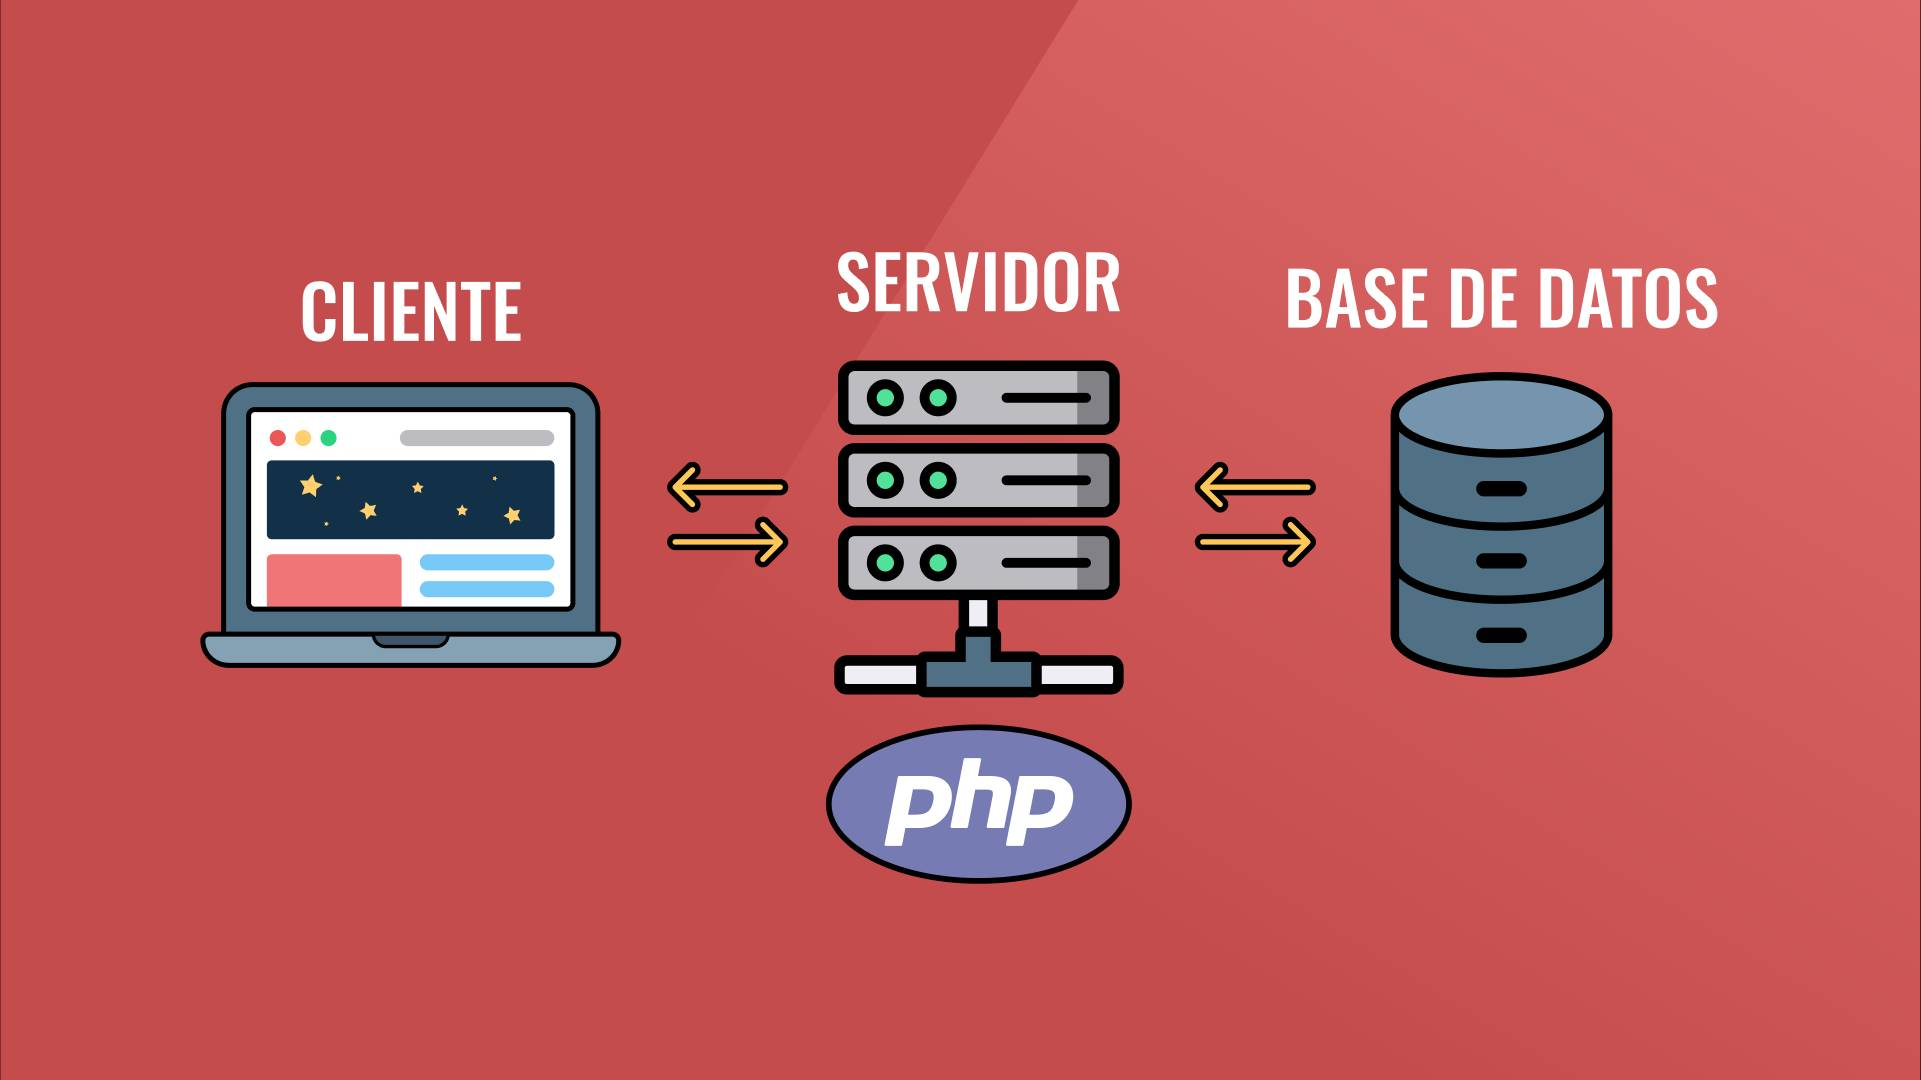
\includegraphics[width=0.5\linewidth]{teorico/backend.jpg}
    \caption{Flujo de un sistema web.}
    \label{fig:Backend}
\end{figure}

Asimismo, el desarrollo back-end desempeña un papel crucial en la seguridad e integridad de los sistemas, ya que de él depende la protección de los datos y la confiabilidad de las transacciones realizadas. Por ello, es fundamental considerar principios como la confidencialidad, la integridad y la disponibilidad de la información, así como la implementación de mecanismos de seguridad adecuados para resguardar los datos durante su almacenamiento y transmisión.

\subsection{.NET}

.NET es una plataforma de desarrollo de código abierto, gratuita y multiplataforma, desarrollada por Microsoft, que permite la creación de una amplia variedad de aplicaciones, incluyendo sistemas web, aplicaciones móviles, de escritorio, videojuegos y soluciones orientadas al Internet de las Cosas (IoT). Esta plataforma soporta múltiples lenguajes de programación, entre los que destacan C\# y Visual Basic, proporcionando un entorno robusto y versátil para el desarrollo de software (Figura \ref{fig:NET}).

\begin{figure}[ht]
    \centering
    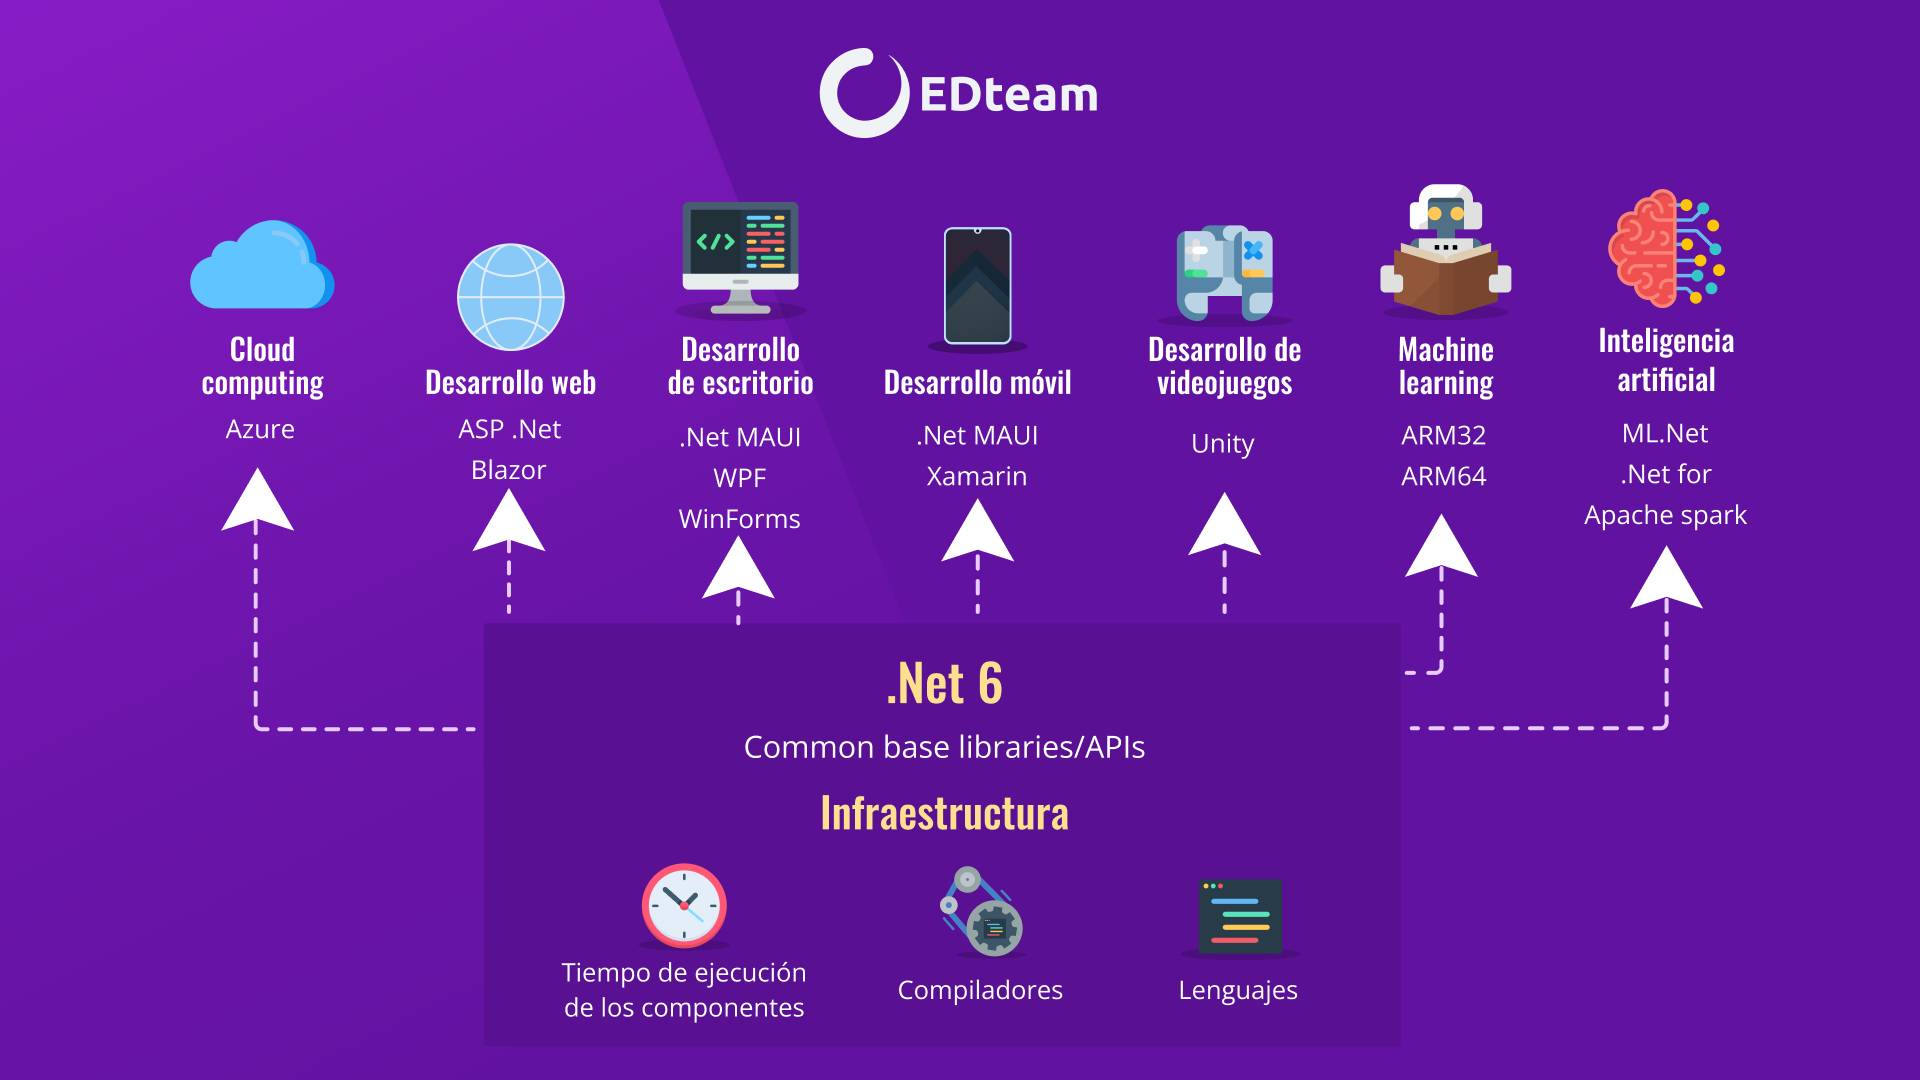
\includegraphics[width=0.5\linewidth]{teorico/net.png}
    \caption{Áreas de utilidad de .NET}
    \label{fig:NET}
\end{figure}

El ecosistema de .NET se caracteriza por su amplia disponibilidad de herramientas que facilitan la integración de funcionalidades adicionales, promoviendo así un desarrollo más ágil, estructurado y mantenible. En el contexto del desarrollo web, .NET es ampliamente utilizado en la construcción del back-end, donde permite implementar la lógica de negocio, la gestión de datos y la exposición de servicios mediante arquitecturas modernas como APIs \parencite[]{Microsoft}.

Gracias a su enfoque en el rendimiento, la seguridad y la escalabilidad, .NET se posiciona como una solución sólida para el desarrollo del núcleo funcional de sistemas web, permitiendo la creación de aplicaciones eficientes y capaces de adaptarse a diferentes entornos y demandas.
 \newpage
\section{Gestores de bases de datos}

Los gestores de bases de datos, también conocidos como sistemas de gestión de bases de datos (Database Management Systems, DBMS), son herramientas diseñadas para facilitar la administración, almacenamiento, consulta y manipulación de datos de manera estructurada \parencite{DBMSGFG}. Estos sistemas actúan como intermediarios entre los usuarios o aplicaciones y los motores de bases de datos, permitiendo una interacción más eficiente y controlada con la información (Ver figura \ref{fig:DBMS}).

\begin{figure}[H]
    \centering
    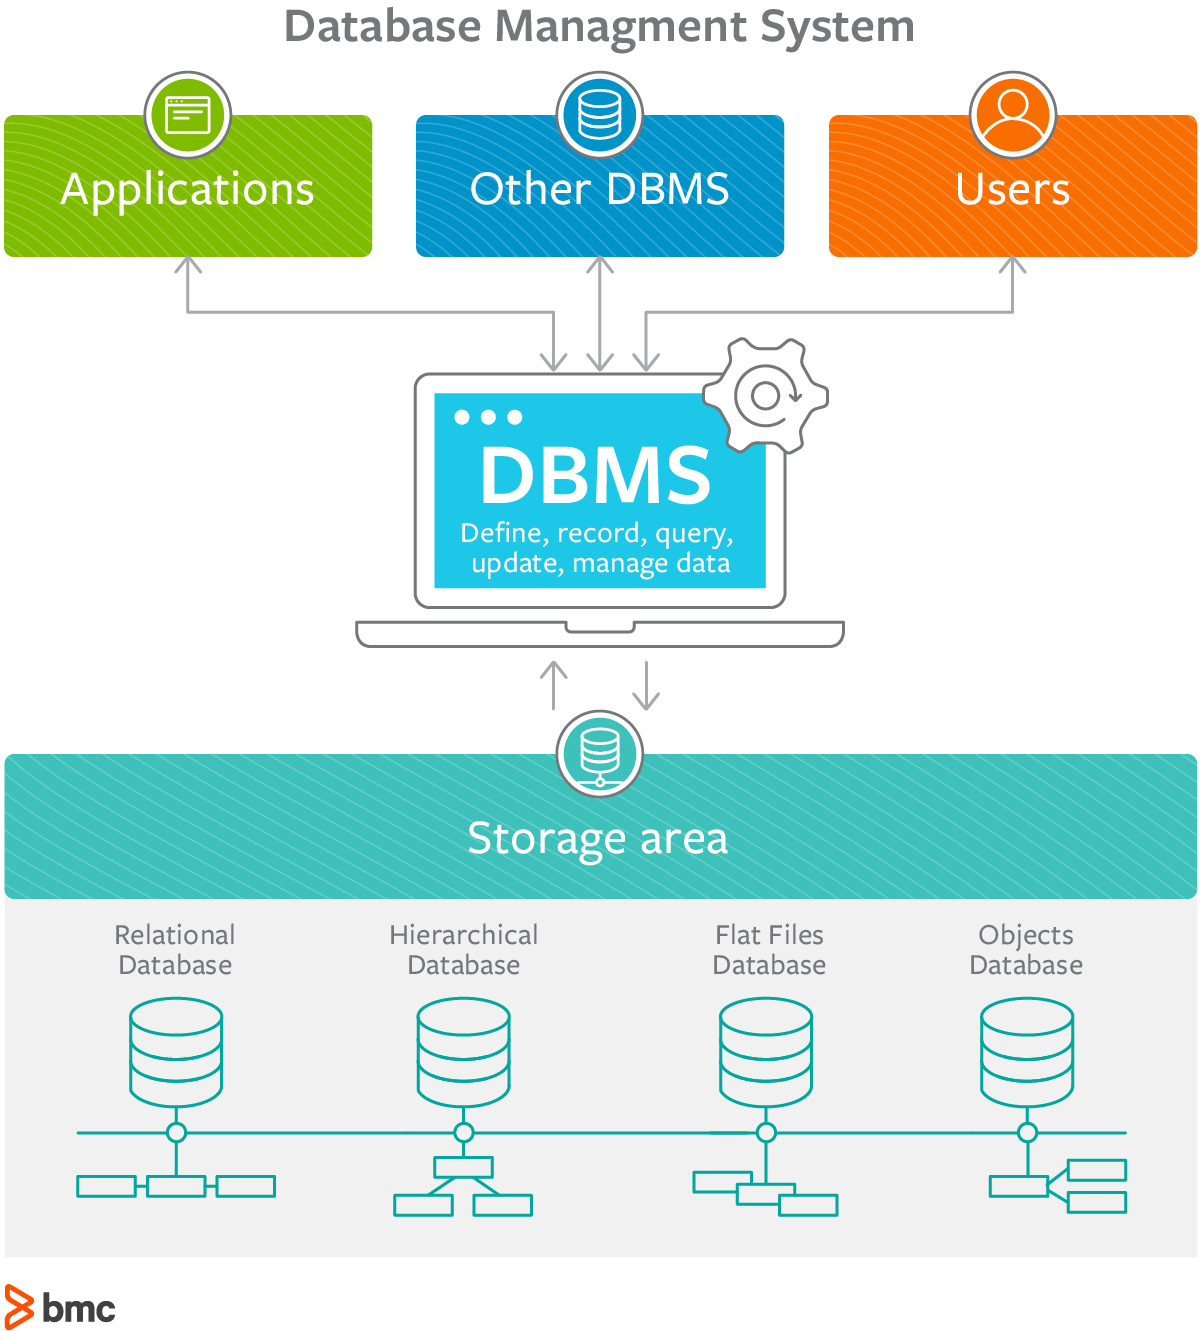
\includegraphics[width=0.5\linewidth]{teorico/dbms.png}
    \caption{Flujo de trabajo de un DBMS.}
    \label{fig:DBMS}
\end{figure}

Su principal objetivo es garantizar la persistencia de los datos a lo largo del tiempo, asegurando características fundamentales como la durabilidad, la integridad y la seguridad de la información. Para ello, los gestores de bases de datos incorporan mecanismos de control de acceso, respaldo, recuperación ante fallos y validación de datos.

Además, estos sistemas permiten gestionar entornos tanto mono-usuario como multiusuario, facilitando el acceso concurrente a la información sin comprometer su consistencia. También ofrecen opciones de configuración y personalización que permiten adaptarlos a las necesidades específicas de cada sistema, favoreciendo su integración dentro de distintas arquitecturas de software.

\subsection{PostgreSQL}

PostgreSQL es un sistema de gestión de bases de datos relacional de código abierto, reconocido por su robustez, extensibilidad y alto rendimiento en el manejo de grandes volúmenes de información. Se ha consolidado como una de las soluciones más utilizadas en la actualidad debido a su capacidad para ejecutar consultas complejas y gestionar datos de manera eficiente y confiable \parencite{PostgreSQL}.

Este gestor se caracteriza por contar con un motor potente que garantiza la integridad, consistencia y seguridad de los datos, además de ofrecer soporte para múltiples tipos de datos, funciones avanzadas y mecanismos de optimización de consultas. Gracias a estas características, PostgreSQL ha sido adoptado por numerosas organizaciones y empresas para el almacenamiento y gestión de información crítica.

PostgreSQL utiliza el lenguaje SQL (Structured Query Language) como medio principal para la definición, manipulación y consulta de datos. A través de este lenguaje, es posible realizar operaciones como inserciones, actualizaciones, eliminaciones y consultas sobre tablas y relaciones, siguiendo el modelo de bases de datos relacionales. Esto permite manejar grandes volúmenes de datos bajo estructuras organizadas, facilitando su acceso y administración de manera eficiente. \newpage

\chapter{Desarrollo de actividades}


\chapter{Resultados finales}
\input{final/DetallesFinales} \newpage
\chapter{Competencias desarrolladas}

Durante la estadía como residente profesional en la empresa TenarisTamsa se adquirieron experiencias en el fortalecimiento de las capacidades profesionales, permitiendo una integración directa con el entorno laboral y proporcionando una visión más amplia sobre los procesos y dinámicas presentes dentro de la industria tecnológica y empresarial. La participación en proyectos reales y en actividades colaborativas dentro del área de Operational Planning IT contribuyó de manera importante al desarrollo tanto técnico como personal, facilitando la adaptación a un entorno profesional enfocado en la resolución de problemas y mejora continua.

Durante el desarrollo del proyecto se aplicaron diversas competencias técnicas adquiridas a lo largo de la formación académica, fortaleciendo conocimientos relacionados con programación, desarrollo de aplicaciones web y estructuración de sistemas de software. Entre las principales habilidades técnicas utilizadas destacan el uso de lenguajes de programación orientados al desarrollo front-end y back-end, la implementación de estructuras de datos, la aplicación de principios de programación orientada a objetos y el manejo de herramientas modernas para la construcción de aplicaciones web.

Asi como el reforzamiento del conocimiento en metodologías ágiles de desarrollo, comprendiendo la importancia de la organización de tareas, seguimiento de actividades y colaboración continua entre los integrantes del equipo para cumplir con los objetivos establecidos dentro de cada fase del proyecto. Esto permitió desarrollar una mayor capacidad de adaptación ante cambios en requerimientos y necesidades operativas del sistema.

De igual manera, el proyecto permitió fortalecer competencias relacionadas con el análisis y resolución de problemas, ya que durante el proceso de desarrollo fue necesario identificar errores, optimizar procesos y proponer soluciones funcionales alineadas con las necesidades del área. Estas actividades favorecieron el pensamiento lógico, la capacidad de investigación y la toma de decisiones técnicas dentro de un entorno de trabajo real.

Por otro lado, también se desarrollaron habilidades blandas fundamentales para el desempeño profesional, tales como la comunicación efectiva, el trabajo en equipo y la colaboración interdisciplinaria. La interacción constante con compañeros del área y con otras áreas involucradas en el desarrollo del sistema permitió mejorar la capacidad para compartir ideas, recibir retroalimentación y coordinar actividades de manera eficiente dentro de un ambiente colaborativo. \newpage
\chapter*{Conclusiones}

El desarrollo de la aplicación web integrada al Sistema Integral de Producción permitió atender las necesidades operativas identificadas dentro de las áreas de producción y ensamblaje de TenarisTamsa, contribuyendo a la modernización y digitalización de procesos relacionados con la gestión de información productiva. A través de la implementación de módulos especializados, se logró fortalecer funcionalidades clave del sistema, mejorando la captura, consulta y administración de datos dentro del entorno operativo.

Durante el desarrollo del proyecto se aplicaron conocimientos relacionados con arquitectura de software, desarrollo frontend y backend, diseño de interfaces, integración de servicios y gestión de bases de datos, utilizando tecnologías modernas como React.js, .NET y PostgreSQL. La implementación de una arquitectura basada en componentes para el frontend y una arquitectura multicapa para el backend permitió desarrollar una solución modular, escalable y mantenible, alineada con los estándares tecnológicos definidos por la organización.

Asimismo, el sistema desarrollado permitió reducir la dependencia de registros manuales, facilitando la disponibilidad de información en tiempo real y mejorando la trazabilidad de los procesos productivos. La centralización de la información y la integración de distintos módulos dentro de una misma plataforma contribuyen a optimizar el seguimiento de órdenes de producción, el control operativo y la toma de decisiones dentro del área de trabajo.

De igual manera, el proyecto permitió reforzar la importancia de las buenas prácticas de desarrollo, documentación y estandarización del código en entornos empresariales e industriales de gran escala. La experiencia obtenida durante el periodo de residencias profesionales favoreció el desarrollo de competencias técnicas y profesionales relacionadas con el trabajo colaborativo, el análisis de requerimientos, la resolución de problemas y la adaptación a procesos corporativos de desarrollo de software.

Finalmente, se concluye que la implementación de soluciones tecnológicas orientadas a la digitalización y automatización de procesos representa un factor clave para mejorar la eficiencia operativa, la confiabilidad de la información y la capacidad de crecimiento de las organizaciones industriales; así como la reducción de la pérdida de información en un 35\% y la disminución del consumo de papel en un 10\%. El sistema desarrollado establece una base sólida para futuras mejoras y ampliaciones dentro del Sistema Integral de Producción, contribuyendo al fortalecimiento tecnológico y operativo de la empresa.

% Referencias bibliográficas
\printbibliography[heading=bibintoc]
\end{document}